
\section[Introduction: Social Modelling]{Introduction: Social Modelling of Artificial Agents \label{Chapter4:Social adaptation}}

The aim of this section is to develop an Agent Based Model which satisfies the
autopoietic property of Social Systems as introduced in the previous
section \ref{Chapter1:SocialSystemTheory}.
The assumption here is that in an Artificial Society
subsystems are formed to reduce uncertainty.
Uncertainty is faced by agents when learning in their environment.
The simplest learning algorithm is an appropriate reflex which
guides the agent from or to a certain object, for example a wall or
food, as described in the previous section \ref{Intro:Braitenberg}. Learning enables the agent to
anticipate reflexes and to generate anticipatory behaviour as discussed in the previous 
section \ref{Introduction:NeuralSystem}. This, however, poses a problem because
when all agents learn, they change their behaviour all the time which
renders them more and more unpredictable to each other \citep{Luhmann95}.
\citet{Luhmann95} proposed that the creation of subsystems will overcome this
problem. Within these subsystems, agents perform more predictably, by
reducing their behavioural complexity. These subsystems are formed by
adaptive communication between the agents which seems to be essential to form
such subsystems.
Both the behaviour and communication is learned by the agent and is not imposed
on the agent.
The goal or motivation of each agent is to collect food, keep it and eat it until
consumed. Every agent broadcasts its hunger state, which can be used by other
agents, into the world.
This results in two subsystems where agents in the
first collect food and in the latter steal food from others.
The section is structured in this way: description of the agents, world and signals involved,
the learning rule used, agents' behaviours, sub-system formation
and effects of different communication strategies followed by a conclusion.

\subsection{Methods: A Model of the World \label{WorldModelSim}}

The simulation model is composed of a 2 dimensional world bounded by walls.
It contains two different objects: agents and food sources.
The agents, referenced by their position as $a_{j}(t)$,where $a_{j}$
has 2 components (x,y coordinates indexed by $a_{j,x}$ and $a_{j,y}$),
with $j=1,..,N$. Agents move with a differential drive system named after
Braitenberg \citep{Braitenberg84}.
Food sources are disks located at fixed position $f_{j}(t)$ with $j=1,...,M$.
They can produce constant food or limited food.

\begin{figure}[htbp]
\begin{center}
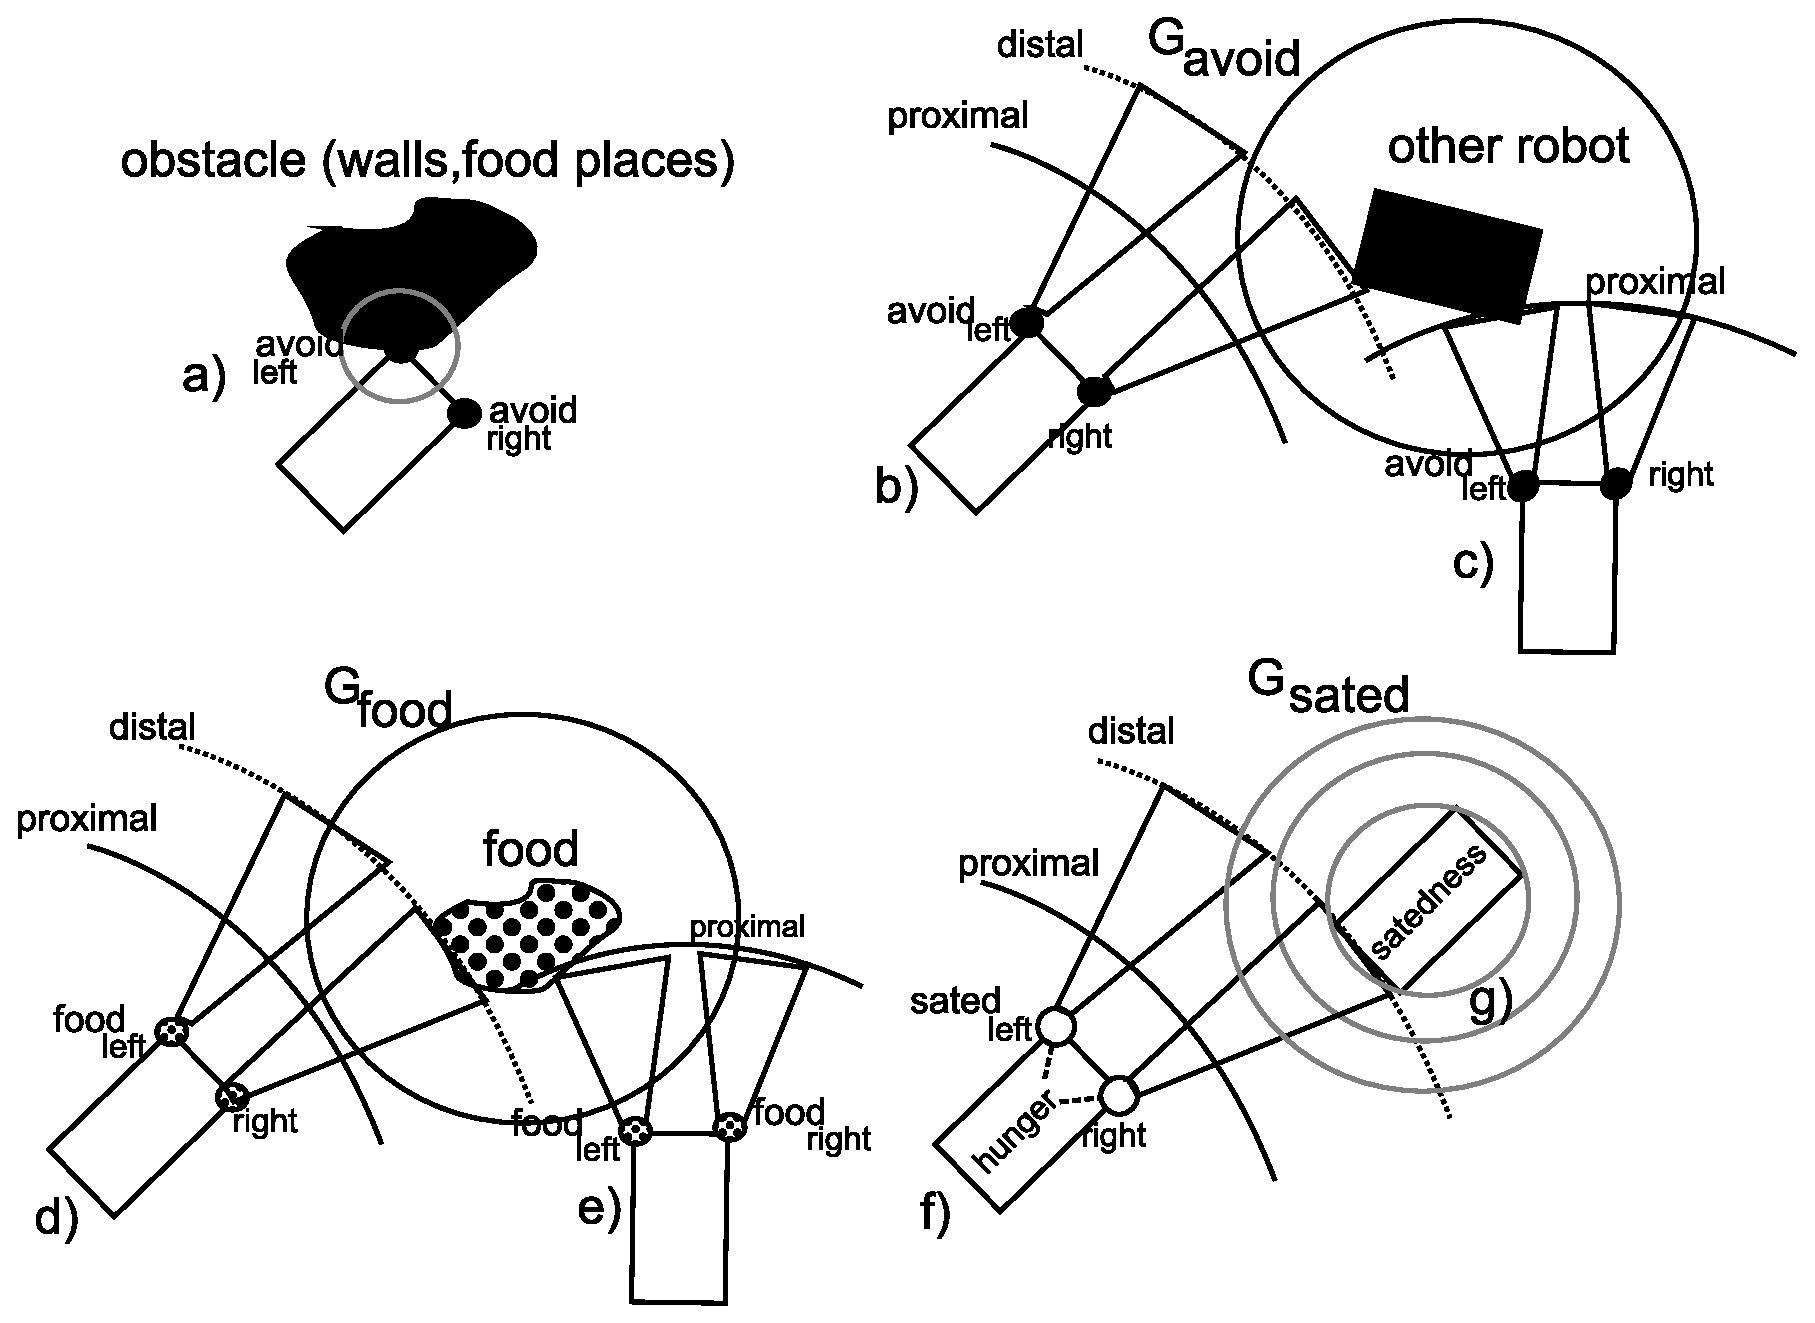
\includegraphics[scale=0.4]{figures/socialadapt/RobotScenario.eps}
\end{center}
\small{
\caption[Social computational model]{Overview of the different signals used in this simulation. 
Circles labelled with G (avoid,food,sated) represent uniform potential fields, circles on 
the robot's front are input sensor, cones irradiating from them represent the field of view 
of sensors, proximal and distal lines represent sensors range. Case a): an agent touches 
a food source or a wall with its proximal left avoidance sensor $avoid_{left,prox}$, 
a proximal signal is generated. Case b): an agent reads the potential field $G_{avoid}$ 
produced by another, with its right distal sensor $avoid_{right,dist}$. Case c): 
an agent reads the potential field $G_{avoid}$ produced by another agent, with 
both left and right proximal sensors $avoid_{left,prox},avoid_{right,prox}$. 
Case d): an agent reads the potential field $G_{food}$ produced by a food source, 
with its right and left distal sensors $food_{right,dist},food_{left,dist}$. 
Case e): an agent reads the potential field $G_{food}$ produced by a close 
food source, with both left and right proximal sensors $food_{left,prox},food_{right,prox}$. 
Case f,g): a hungry agent f (with $Hunger=1$) reads the satedness signal $G_{sated}$ 
produced by the sated agent g. \label{fig:sensors}
}}
\end{figure}

Agents have different sensors which enable them to sense
obstacles, other agents' presence and others' broadcasted state of satedness, at
different ranges (proximal and distal see Fig. \ref{fig:sensors}).
Every object labelled with a certain index $j$ produces a signal carried by a
uniform potential field $G_{j,type}$ with a limited range, which is sensed
by the corresponding sensor type (type can be avoid,food or sated).
The potential field $G_{j,type}$ is described by the equation of a circle which is centered
on $x_0,y_0$ with a $r$ radius:
\begin{equation}
(x-x_0)^2+(y-y_0)^2=r^2 \label{eq:circle}
\end{equation}
Every geometric point $x,y$ including a sensor or object which falls inside 
the circle $G_{j,type}$ assumes a unitary value.
The signals from the proximal sensors ($x_{0}$) are originally used to drive
the agents reflexes which can either be avoidance or attraction. The signals
from the distal sensors are used for learning so that the agent is able to
generate anticipatory reactions instead of the reflexes as introduced in section \ref{Introduction:NeuralSystem}.

In the next section I am going to describe the learning algorithm enabling the agent to
replace the reflexes with the predictive actions.
Once the learning algorithm is described, I will describe the different reflexes and possible
anticipatory reactions.
\subsection{Methods: ICO learning module \label{Section:ICOlearning}}

The input correlation learning rule of \citet{Porr2006ICO} is a Hebbian learning rule,
it is unsupervised and performs a confounded correlation between a predefined reflex signal
($x_{0}$) and a reflex predicting signal ($x_{1}$). Hence, this learning
algorithm identifies and exploits causalities between temporal
sequential signals.
The ICO learning block was chosen because it is one of the simplest,fastest and computationally 
efficient approach to temporal learning.
It can also be easily implemented in analogic and digital systems without any
 particular modifications.

\begin{figure}[htbp]
\begin{center}
\includegraphics[scale=0.5]{figures/socialadapt/ico.eps}
\caption[Agent learns with the ICO learning]{Figure (a) shows the ICO learning basic
block composed by 2 inputs $x_{0},x_{1}$ filtered by $h_{0},h_{1}$ and the output $v$.
Figure (b) shows the weight change of $w_{1}$ during time. At the beginning $w_{1}=0$,
then for 5000 simulation steps $x_{1}$ anticipates $x_{0}$ and the $w_{1}$ grows until 1.0.
After 5000 simulation steps reflex is suppressed $x_{0}=0$ and $w_{1}$ stabilises to $1 \cdot 10^{-3}$.
\label{fig:ico}}
\end{center}
\end{figure}

Figure \ref{fig:ico} shows the ICO learning block which has two inputs $x_{0}$,$x_{1}$
from the agent's sensor that are filtered by low pass filters $h_{0},h_{1}$:

\begin{eqnarray}
&h(t)=&\frac{1}{b}e^{at}sin(bt) \label{eq:1}\\
&a   =&-\pi \frac{F}{Q} \label{eq:F}\\
&b   =&\sqrt{(2\pi F)^2 -a^{2}} \label{eq:Q}
\end{eqnarray}

$F$ is the oscillation frequency and $Q$ the quality factor. The low passed
signals $u_{i}(t)$ are transferred with weight $w_{i}$ to the output
neurons (for more details see Appendix \ref{app:appendixICO}).

\begin{eqnarray}
u_1 &=& h \ast x_1 \\
u_0 &=& h \ast x_0
\end{eqnarray}

where $\ast$ is the convolution operation which implement the filtering operation.
In the output neuron the output $v(t)$ is calculated by
summing up all incoming signals according to their weights:
\begin{equation}
v(t)=w_{0}\cdot u_{0}+w_{1}\cdot u_{1}
\end{equation}
which represent the input for the motor system.
The unsupervised character of the ICO learning rule is reached by
the synaptic weight $w_{1}$ to be adapted by the weight
change rule:
\begin{equation}
\frac{\partial w_{1}}{\partial t}=\mu u_{1} \frac{\partial u_{0}}{\partial t}
\end{equation}
The weight change is dependent on the derivative of the reflex input
signal $u_{0}$, the input signal $u_{1}$ and a
learning rate $\mu$. The
learning rule has been shown to be useful for avoidance and attraction
mechanisms and has fast and stable convergence.


\subsection{Methods: agent controller}
For the sake of simplicity, the agent's neural controller is analysed block
by block according to the requested behaviours (avoidance and attraction)
in Figs. \ref{fig:avoidance},\ref{fig:attractionAgent},\ref{fig:attraction}.
The core is composed of two ICO neurons, labelled with L-eft and R-ight,
connected to the motor outputs left and right. Both ICO neurons have a
constant bias input B with weight 4.0 that makes the robot move forward
if inputs are absent. Rectangular blocks labelled with L,R are low pass
filters, with parameters $F,Q$ referred to equations \ref{eq:F},\ref{eq:Q}.
Synaptic weights of the ICO block in Fig. \ref{fig:ico}(a) are labelled with
$W$ capital letter and two pedex that indicate the weight type
(predict is learned and reflex is fixed) and the synapse position (left,right).
ICO neurons have recurrent synaptic connections, labelled as
$W_{R2L},W_{L2R},W_{selfR},W_{selfL}$ to implement a hysteresis effect,
which causes the controller to not instantly follow signals (as in \citealt{Hulse2004,Paseman2002}).
It means reactions on an incoming signal are time shifted. This is useful to enable agents to escape from acute angles: if
an agent incurs in an concave acute angle and has not a hysteresis mechanism,
will get stuck inside, turning left and right alternatively.

\subsection{Methods: avoidance behaviour}
Agents and walls are obstacles. Agents produce obstacle
signals (see Fig.\ref{fig:sensors} (a) for obstacles and
Fig.\ref{fig:sensors} (b),(c) for other agents). Every agent $a_{j}(t)$ has a
potential field associated (see Eq.\ref{eq:circle}):
\begin{equation}
Gavoid_{j}(t)=G(x-a_{j,x}(t),y-a_{j,y}(t)).
\end{equation}
that is sensed by the corresponding inputs of other agents $a_{k}(t)$ (with $k\neq j$)
labelled as $avoid_{left,right}$. Walls and food sources
do not produce $G_{avoid}$, so that agents sense them using proximal signals that are
generated by collisions: when 2 distinct agents $j$ and $l$ collide at time $t_{0}$, such
that $||a_{j}(t)-a_{l}(t)||_{2}<D$ ($D$ is the radius of the
agent) an impulse is produced at $avoid_{l,r}$.
\begin{figure}[htb]
\begin{center}
\includegraphics[scale=0.45]{figures/socialadapt/avoidance.eps}
\end{center}
\vspace*{4pt}
\small{
\caption[Avoidance learning behaviour]{Avoidance network: ICO left and right are
two neurons implementing the ICO learning rule, their output is a sigmoid and
is connected (after normalization into $[v_{min},v_{max}]$) to the motor speed commands.
Grey triangles represents distal inputs, while white triangles represent proximal inputs.
The learned synaptic weights are associated to the distal synapses (thick lines) while
the fixed are associated to the proximal synapses (dotted lines).
To produce a retraction behaviour left and right weights must be different
such that
$W_{predict,L}>W_{predict,R}$ and $W_{reflex,L}>W_{reflex,R}$, if
$W_{predict,L}=W_{predict,R}$ and $W_{reflex,L}=W_{reflex,R}$ robot
will just go back without turning.\label{fig:avoidance}}}
\end{figure}
The neural controller for the avoidance behaviour is shown in
Fig. \ref{fig:avoidance} (see also \citealt{Stamm2006}), every ICO neuron (left and right)
computes the following operations:

\begin{eqnarray}
ICO_{L}(t)&=B-h \ast avoid_r\cdot W_{reflexL}-h \ast avoid_{dist,r}\cdot W_{predictL}\\ \nonumber
	  &+W_{selfL}\cdot ICO_{L}(t-1) + W_{L2R}\cdot ICO_{R}(t) \label{eq:ICO:L1} \\ 
ICO_{R}(t)&=B-h \ast avoid_l\cdot W_{reflexR}-h \ast avoid_{dist,l}\cdot W_{predictR}\\ \nonumber
	  &+W_{selfR}\cdot ICO_{R}(t-1) + W_{R2}\cdot ICO_{L}(t)  \label{eq:ICO:R1}
\end{eqnarray}

The parameters used for the weights, the bias and the recurrent connections are
reported in the Appendix sections \ref{Appendix:HysteresysValue},\ref{Appendix:simulation}.
The recurrent connections between the left and right ICO neuron, are necessary
to implement a push-pull behaviour so that when the robot synchronously activates
both the left and the right input, only one ICO neuron will dominate thus evoking
a turn-back response. 
Connections between input synapses and ICO neurons (motor neurons) are
negative to evoke a retraction. 
The motor output is calculated with a sigmoid activation function on the ICO neuron
membrane as follow:

\begin{eqnarray}
V_{L}&=& \frac{1}{1+e^{-ICO_{L}}}\\
V_{R}&=& \frac{1}{1+e^{-ICO_{R}}}
\end{eqnarray}

The weight update learning rule is calculated for the weigts:

\begin{eqnarray}
\frac{\partial W_{predict,L}}{\partial t}&=& \mu \cdot avoid_{dist,l} \frac{\partial avoid_{l}}{\partial t}\\
\frac{\partial W_{predict,R}}{\partial t}&=& \mu \cdot avoid_{dist,r} \frac{\partial avoid_{r}}{\partial t}
\end{eqnarray}


\subsection{Methods: Agents and satedness communication}
Every agent has an internal state: hunger and its complementary satedness.
\begin{figure}[htbp]
\begin{center}
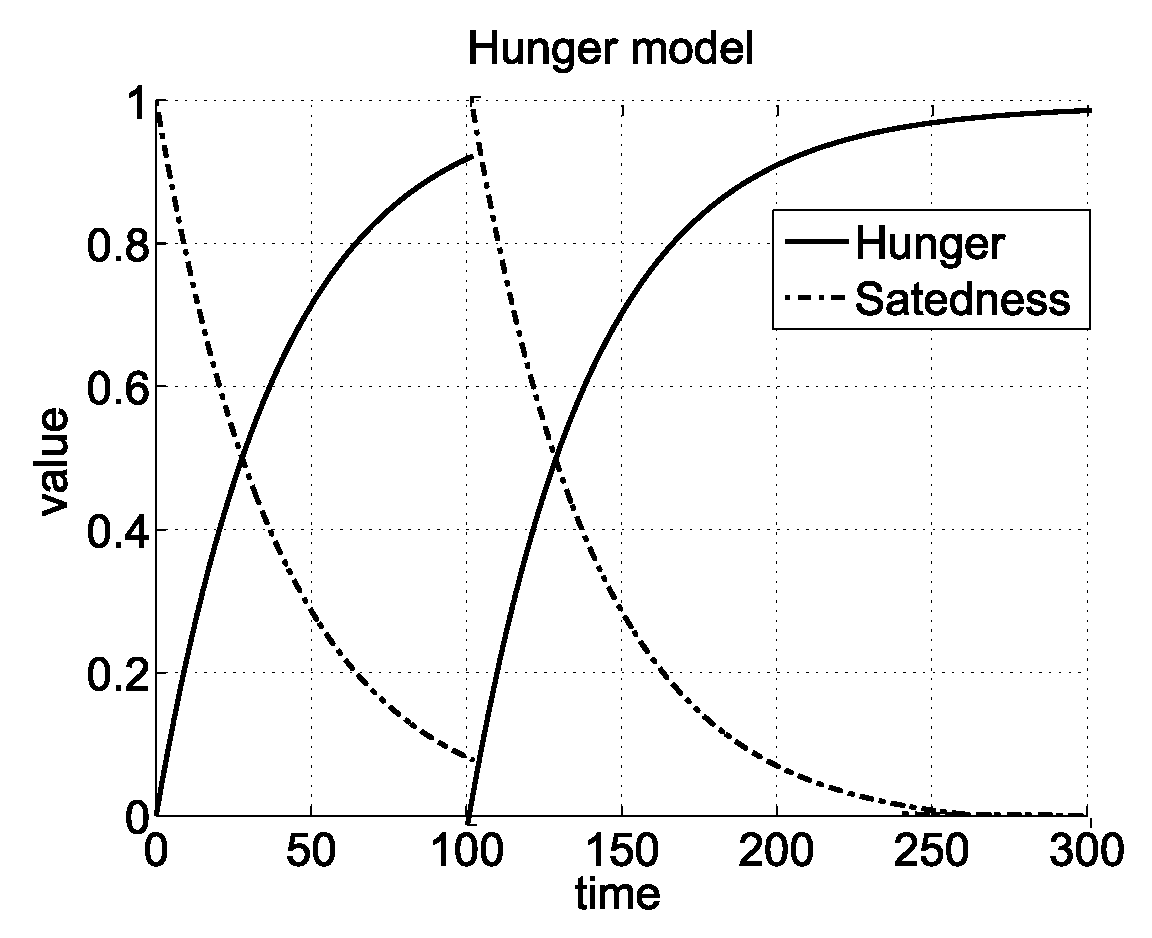
\includegraphics[scale=0.3]{figures/socialadapt/hungersatshift.eps}
\end{center}
\vspace*{4pt}
\caption[Energy state or hunger of the artificial agent]{
Hunger state in function of time. At time step 100 the agent touches a
food place, thus its hunger state is reset to 0 and so its complementary
satedness to 1. \label{fig:hunger}}
\end{figure}

The energy level of each agent is an exponential function of time:
\begin{equation}
H_{sated}(t)=
  \begin{cases}
   e^{-t/\tau_{starv}} & \text{if } t \geq t_b \\
   0       & \text{if } t < t_b
  \end{cases}
\label{eq:satstate}
\end{equation}
and complementary its hunger state is:
\begin{equation}
H_{hunger}(t)=1-H_{sated}(t)
\end{equation}
where $\tau_{starv}$ is the starvation factor and $t_b$ corresponds to the moment
when an agent touches a food source:
\begin{equation}
|food_{l,prox,d_{1}}(t_{b})+food_{r,prox,d_{1}}(t_{b})|>\theta_{F}
\label{eq:touchfood}
\end{equation}
or touches a sated agent (see Fig. \ref{fig:hunger}):
\begin{equation}
|sated_{l,prox,d_{1}}(t_{b})+sated_{r,prox,d_{1}}(t_{b})|>\theta_{A}
\label{eq:touchagent}
\end{equation}
and agent is touching an obstacle
\begin{equation}
|avoid_{prox,l}(t_{b})+avoid_{prox,r}(t_{b})|>\theta_{O}
\end{equation}
where $\theta_{F},\theta_{A},\theta_{O}$ are thresholds for food, agents and
obstacles respectively.
In Fig. \ref{fig:attractionAgent}, internal state $H_{hunger}(t)$ is multiplied
for $food(t)$ (left,right and proximal,distal) and $sated(t)$ (left, right and proximal, distal).

Satedness internal state of agent $a_{i}$, is broadcasted to other agents
$a_{k}(t)$ (with $k\neq j$) by means of a potential field (see Fig.\ref{fig:sensors}(g) and Eq.\ref{eq:circle}):
\begin{equation}
G_{i,sated}(t)=H_{sated}(t) \cdot G(x-a_{i,0},y-a_{i,1}).
\label{eq:gsated}
\end{equation}
Agent $a_{k}(t)$ senses $G_{i,sated}$ (see Fig.\ref{fig:sensors} (f)) with 2
reflexive inputs $sated_{l,prox,d_{1}}(t)$ and 
$sated_{r,prox,d_{1}}(t)$ whose difference feeds the reflexive input:
\begin{equation}
x_{0}(t)=sated_{l,prox,d_{1}}(t) - sated_{r,prox,d_{1}}(t).
\end{equation}
and as predictive $sated_{l,prox,d_{2}}(t),sated_{r,prox,d_{2}}(t)$ whose
difference feeds the predictive input:
\begin{equation}
x_{1}(t)=sated_{l,dist,d_{2}}(t) - sated_{r,dist,d_{2}}(t).
\label{eq:foodagentpredictive}
\end{equation}
where $d_{2}>d_{1}$.
The equations \ref{eq:ICO:L1},\ref{eq:ICO:R1} of the ICO neurons are added to the
following synaptic inputs:

\begin{eqnarray}
ICO_{L}&=&-h \ast ( x_0 \cdot H_{hunger}) \cdot W_{reflex,A,L} \\ \nonumber
       & &-h \ast ( x_1 \cdot H_{hunger}) \cdot W_{predict,A,L} \label{eq:ICO:L2}\\
ICO_{R}&=& h \ast ( x_0 \cdot H_{hunger}) \cdot W_{reflex,A,R} \\ \nonumber
       & &+h \ast ( x_1 \cdot H_{hunger}) \cdot W_{predict,A,R} \label{eq:ICO:R2}
\end{eqnarray}
The reason for the sign inversion for the weights is that the inputs
are differential and thus is necessary for the left ICO neuron have
an input of opposite sign to the right ICO neuron.
The weight update rule this time is:
\begin{eqnarray}
\frac{\partial W_{predict,A,L}}{\partial t}&=& \mu \cdot x_1 \frac{\partial x_0}{\partial t}\\
\frac{\partial W_{predict,A,R}}{\partial t}&=& \mu \cdot x_1 \frac{\partial x_0}{\partial t}
\end{eqnarray}

Inputs for the attraction task are shown in Fig. \ref{fig:attractionAgent}.
When for example:  $x_{0}(t)>0$ implies that a sated agent is on the left
$sated_{l,prox,d_{1}}(t)>0$, the neural controller produces $v_{L}<v_{R}$,
agents turns left until $x_{0}(t)=0$ that means either $x_{0}(t)=x_{1}(t)$
(a sated agent is in front) or $x_{0}(t)=x_{1}(t)=0$ (no sated agent in front).
A hungry agent, is producing $G_{i,sated}(t)=0$ therefore other agents will be
 repelled since it is emitting only the $G_{avoid}$ signal.

\paragraph{Aggressive agents}
If one wants to make an agent more aggressive $H_{sated}(t)$ can be multiplied for the
distal sensors $avoid(t)$ left, right (in Fig.\label{fig:avoid} the $H_{hunger}$
block can be introduced after each of the grey triangles). 
\begin{equation}
H_{sated}(t)\cdot avoid(t)  \label{eq:aggressive}
\end{equation}
It implies that when an agent is not sated, it will ignore the obstacle
signal $G_{avoid}$ produced by the other agent.

\begin{figure}[htb]
\includegraphics[scale=0.4]{figures/socialadapt/attractionAgent.eps}
\small{
\caption[Attractive behaviour for other agents]{
Attraction toward sated agents:two more inputs are added to the ico neurons.
Grey triangles represents distal inputs, while white triangles represent
proximal inputs. The learned synaptic weights are associated to the distal
synapses (thick lines) while the fixed are associated to the proximal
synapses (dotted lines). Synaptic weights must be equal in module and
opposite in sign $|W_{predict,A,L}|=|W_{predict,A,R}|$ and
$|W_{reflex,A,L}|=|W_{reflex,A,R}|$  where $A=agent$.
Hunger internal state is multiplied for proximal and distal
input difference \label{fig:attractionAgent}}
}

\end{figure}


\subsection{Methods: Food attraction}
Every food source $f_{j}(t)$ with $j=1,...,M$ produces the signal
(see Fig.\ref{fig:sensors} (d),(e) and Eq.\ref{eq:circle}):
\begin{equation}
G_{j,food}=G(x-f_{j,x},y-f_{j,y})
\label{eq:food}
\end{equation}
which is sensed by agents $a_{i}$ by the inputs labelled as
$food_{left,right}$ (see Fig.\ref{fig:sensors} (d),(e)).
\paragraph{Constant food production}
Every food source contains a constant amount of food which means $G_{j,food}$
is always emitted.
\paragraph{Limited food production}
Every food source contains a limited amount of food modelled by the variable $q$ that
 is decremented every time an agent touches the food place at $t_{b}$:
\begin{equation}
q_{j}(t_{b}+1)=q_{j}(t_{b})-\theta q
\label{eq:qfood}
\end{equation}
where ($\theta q$ is fixed).
When $q_{j}=0$ the food source $j$ is exhausted and food signal is suppressed $G_{j,food}=0$.
After a random period the food source is restored $q_{j}=1$.
\begin{figure}[htb]
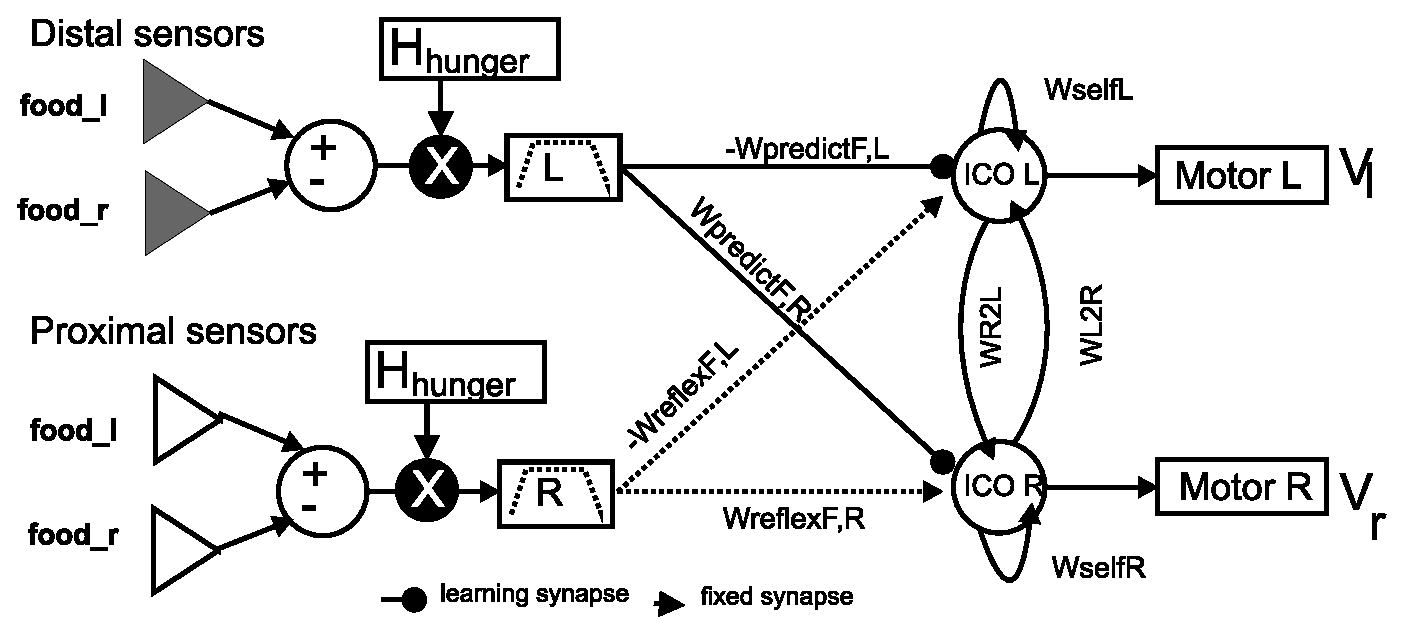
\includegraphics[scale=0.4]{figures/socialadapt/attractionFood.eps}
\vspace*{4pt}
\small{
\caption[Attraction learning behaviour for food]{Attraction toward food:
two more inputs are added to the previous network. Grey triangles represents
distal inputs, while white triangles represent proximal inputs.
The learned synaptic weights are associated to the distal synapses (thick lines)
 while the fixed are associated to the proximal synapses (dotted lines).
Synaptic weights in the attraction task must be equal in module and opposite
in sign: $W_{predict,F,L}=W_{predict,F,R}$ and $W_{reflex,F,L}=-W_{reflex,F,R}$
where $F=food$ \label{fig:attraction}}
}
\end{figure}

Required inputs for the attraction behaviour are introduced in
Fig. \ref{fig:attraction} (see also \citealt{Stamm2006}),
for every ICO neuron an additional reflex is added:
\begin{equation}
x_{0}(t)=food_{l,prox,d_{1}}(t)-food_{r,prox,d_{1}}(t).
\end{equation}
$x_{0}$ it is the difference between the left and right proximal food input sensors.
A predictive input is added:
\begin{equation}
x_{1}(t)=food_{l,dist,d_{2}}-food_{r,dist,d_{2}}(t).
\end{equation}
$x_{1}(t)$ it is the difference between the left and right distal food input sensors.
Thus $d_{2}>d_{1}$ such that the distal food sensor values are
predictive on the proximal food sensors.
The equations \ref{eq:ICO:L2},\ref{eq:ICO:R2} of the ICO neurons are added to the
following synaptic inputs:

\begin{eqnarray}
ICO_{L}&=&-h \ast ( x_0 \cdot H_{hunger}) \cdot W_{reflex,A,L} \\ \nonumber
       & &-h \ast ( x_1 \cdot H_{hunger}) \cdot W_{predict,A,L} \label{eq:ICO:L3}\\
ICO_{R}&=& h \ast ( x_0 \cdot H_{hunger}) \cdot W_{reflex,A,R} \\ \nonumber
       & &+h \ast ( x_1 \cdot H_{hunger}) \cdot W_{predict,A,R} \label{eq:ICO:R3}
\end{eqnarray}
The reason for the sign inversion for the weights is that the inputs
are differential and thus is necessary for the left ICO neuron have
an input of opposite sign to the right ICO neuron.
The weight update rule this time is:
\begin{eqnarray}
\frac{\partial W_{predict,A,L}}{\partial t}&=& \mu \cdot x_1 \frac{\partial x_0}{\partial t}\\
\frac{\partial W_{predict,A,R}}{\partial t}&=& \mu \cdot x_1 \frac{\partial x_0}{\partial t}
\end{eqnarray}

When for example: $x_{0}(t)>0$ implies that food source is on the left, the neural
controller produces $v_{L}<v_{R}$, agent turns left until $x_{0}(t)$ becomes 0.

\subsection{Controller summary}
For clarity Fig. \ref{fig:controllerSummary} contains the simplified but full structure of the controller whereby the two
ICO neurons receive synaptic inputs from each synaptic input described before.
There are a total of twelve inputs because for every behaviour there are left and
right sensors for the distal and proximal case.
Because there are three behaviours, multiplied by 4 makes 12 parallel inputs.
The inputs are then low pass filtered as described before and summed at the 
ICO neuron $\sum$.
The left and right ICO neurons are also responsible for updating the weights
for the predictors.
The output of each ICO neuron is then fed into a sigmoid function which normalizes
the output in the $[-1,1]$ range for controlling the robot motors.

\begin{figure}
\begin{center}
\includegraphics[width=1.0\textwidth]{figures/socialadapt/ControllerSummary}
\end{center}
\vspace*{4pt}
\caption[Full schematic of the controller]{
The robot controller implements the 3 behaviours by using a linear
summation of all the synaptic inputs \label{fig:controllerSummary}}
\end{figure}


\subsection{Broadcasting signal mechanism \label{SocialSystem:Broadcast}}

The main feature of a social system is the production and use of signals.
Thus each agent can emit the same field in equation \ref{eq:food} in the presence of a food source.
A more detailed discussion about signalling strategies is in the Conclusion section \ref{TheoryOfMind}.
There are only two possible signalling strategies in my model, honest and dishonest
strategies and are going to be described in the following sections.

\subsubsection{Honest food proximal signalling}
In this scenario agents signal the presence of food when they sense it using
the proximal inputs: $G_{food}$ is emitted by an agent when $food_{l,prox,d_{1}}(t)>0$, $food_{r,prox,d_{1}}>0$
and $|food_{l,prox,d_{1}}(t)-food_{r,prox,d_{1}}|<\theta F$ ($\theta F$ as Eq.\ref{eq:touchfood}).
This "genuine" social behaviour might increase the foraging performance of the colony,
but might cost the signaller because it can result in higher robot density and increased
competition and interference nearby the food (i.e. spatial constraints around the food disk:
only 9 agents can forage at same time). Thus, although beneficial to other colony members,
signalling of a food location can constitute a costly act \citep{AnimalSignals} because it
decreases the food intake of signalling robots. With this social rule agents tend to form
lines around the food zones: they are more organized then the previous case.

\subsubsection{Dishonest food proximal signalling}
In this case the agent "cheats" producing non predictable (using a uniform probability
of emitting $p(e)=0.6$) food signals when they are far away from the food zones
($food_{l,dist,d_{2}}=0$ AND $food_{r,dist,d_{2}}(t)=0$) and of course when they
are not sated ($H_{sated}(t)< 0.2$ a threshold). The percentage of cheaters used in the
test was: $10\%,50\%$,and $80\%$. Doing so an agent reduces the competition around the food zones.


\subsection{Results: analysis of formation in different cases}
The following sections contain the most important test cases for our model:
\begin{itemize}
\item general overview about the sub-system property and the food signalling strategies
\item a comparison of the food performance between adaptive communication and non communicative strategy
\item an insight to the honest behaviour with unlimited resources
\item an insight to the honest behaviour with limited resources and environmental changes
\end{itemize}

\subsubsection{Sub-system formation and adaptive communication}
During time agents learn to: avoid obstacles, search for food and search for
other sated agents.
Because all the inputs (see Fig. \ref{fig:controllerSummary}) are used in parallel
and summed linearly for the motor behaviour, the weights will develop independently
from each other in a competitive fashion.
For example when an agent sees a closer agent with food and a food source, the outcome
of the motor behaviour will depend on the weight status for each behaviour.
Thus agents can be classified in 2 classes, seekers and parasites,
according to their weights \footnote{$W_{predict,A}$ is the average
of $|W_{predict,A,L}|,|W_{predict,A,R}|$ and $W_{predict,F}$ is the average of $|W_{predict,F,L}|,|W_{predict,F,R}|$}:
\begin{equation}
\delta_{w,agent}=\frac{|W_{predict,A}(0)-W_{predict,A}(T_{sim})|}{W_{predict,A}(0)}.
\end{equation}

\begin{equation}
\delta_{w,food}=\frac{|W_{predict,F}(0)-W_{predict,F}(T_{sim})|}{W_{predict,F}(0)}.
\end{equation}

where the fraction is used to normalize the weight development, so in summary:
\begin{itemize}
 \item \textbf{An agent is a seeker} $\delta_{w,agent} > \delta_{w,food}$, if it is more
attracted by food places than other sated agents.
\item \textbf{An agent is a parasite} $\delta_{w,agent}\leq \delta_{w,food}$, if it is
more attracted by sated agents than food places.
\end{itemize}
This classification will then be compared to a subjective comparative analysis in
section \ref{Chapter8:PPsocial} where the Predictive Performance will allow the 
sub system analysis withouth the need of comparing the weights on each agent.

Sub-system formation is analysed for 2 important test cases:
\begin{itemize}
 \item adaptive communication: the agents learn using both proximal and distal signals
 \item no communication: the agents do no produce the $G_{sated}$ food signal necessary
for the other agents to know whether food is available or not.
\end{itemize}
The non communicative condition does not imply that in Eq. \ref{eq:foodagentpredictive} distal
signals are suppressed but rather that agents will learn only when the neighbouring agent
is enough close to be sensed by the far sensors.
This implicate that learning will be happening still but only when robots are close 
to each other rather than via the broadcast field  $G_{sated}$.
For our simulation, a population of $N=20$ agents is provided with $M=4,10,18$ food sources sequentially.
Population dynamic is observed for a total duration of  $T_{sim}=80000$ (time step $\triangle T=0.01 s$).
Fig.\ref{fig:generalcomparison} resumes a total of 6 test cases: left column considers scarce resources
 ($M=4$ food sources against $N=20$ agents), right column considers abundant resources ($M=18$ food sources against $N=20$ agents).
Each one of them reports the number of seekers (thick line) and parasites (dotted line) in function of time.
The number of seekers $n_{s}(t)$ is complementary to the number of parasites $n_{p}(t)$: 
\begin{equation}
n_{s}(t)+n_{p}(t)=N \label{eq:social:ratio} 
\end{equation}
When the simulation is over $t=T_{sim}$ the ratio is:
\begin{equation}
n_{s}(T_{sim})+n_{p}(T_{sim})=N \label{eq:social:ratiofin} 
\end{equation}

\begin{figure}[htbp]
  \begin{center}
      \subfigure[No food signal, ratio $N=20,M=4$]{
	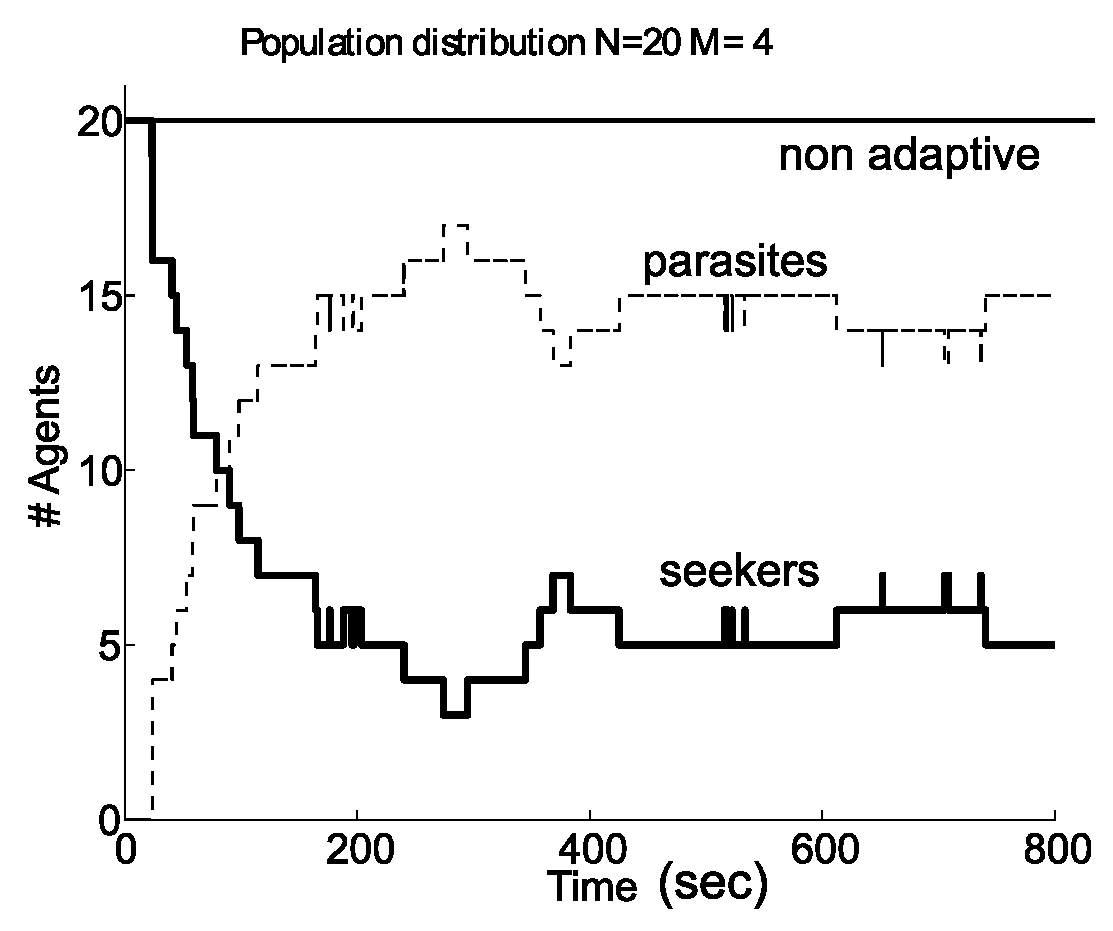
\includegraphics[width=0.4 \textwidth]{figures/socialadapt/nosignal/comm20TO4.eps}}
      \hspace{1pt}
      \subfigure[No food signal, ratio $N=20,M=16$]{
	\includegraphics[width=0.4 \textwidth]{figures/socialadapt/nosignal/comm20TO18.eps}}
      \vspace{1pt}
      \subfigure[Honest food signal, ratio $N=20,M=4$]{
	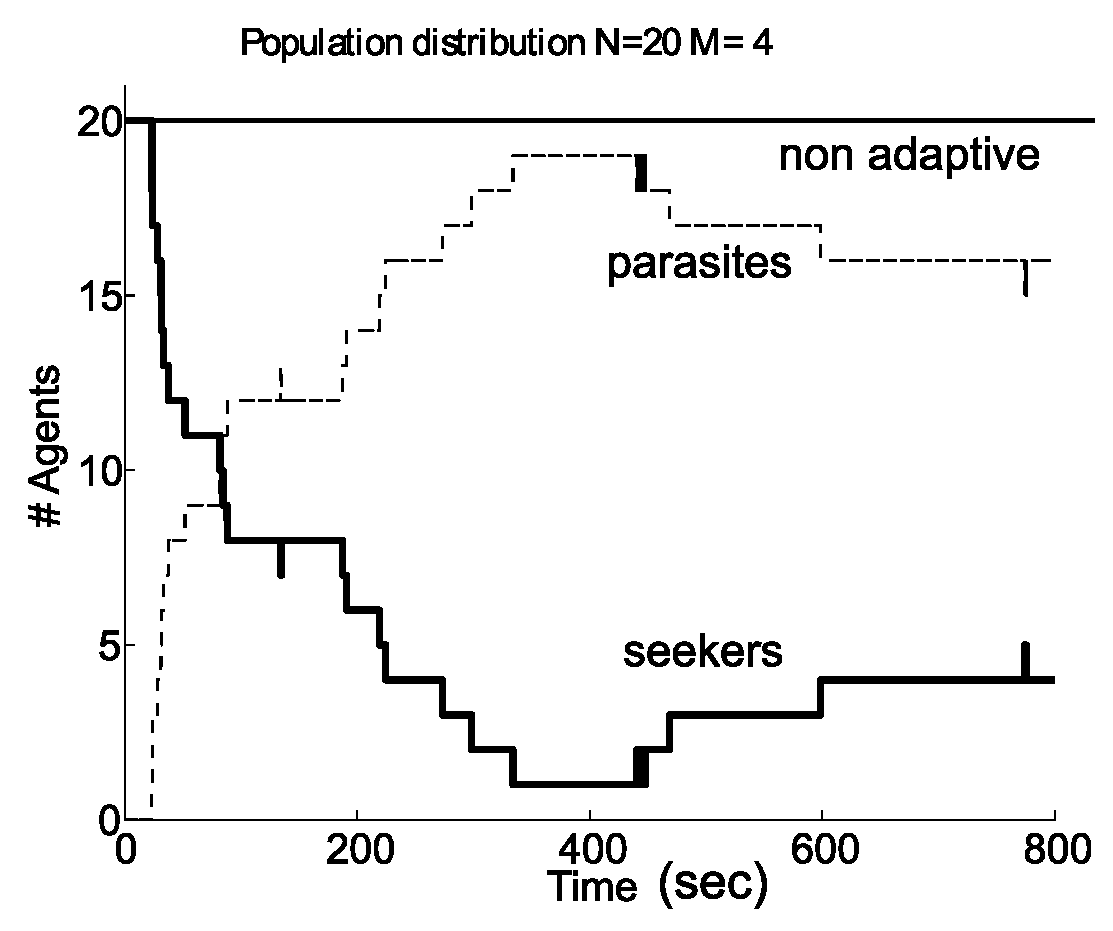
\includegraphics[width=0.4 \textwidth]{figures/socialadapt/honest/comm20TO4.eps}}
	\hspace{1pt}
      \subfigure[Honest food signal, ratio $N=20,M=16$]{
	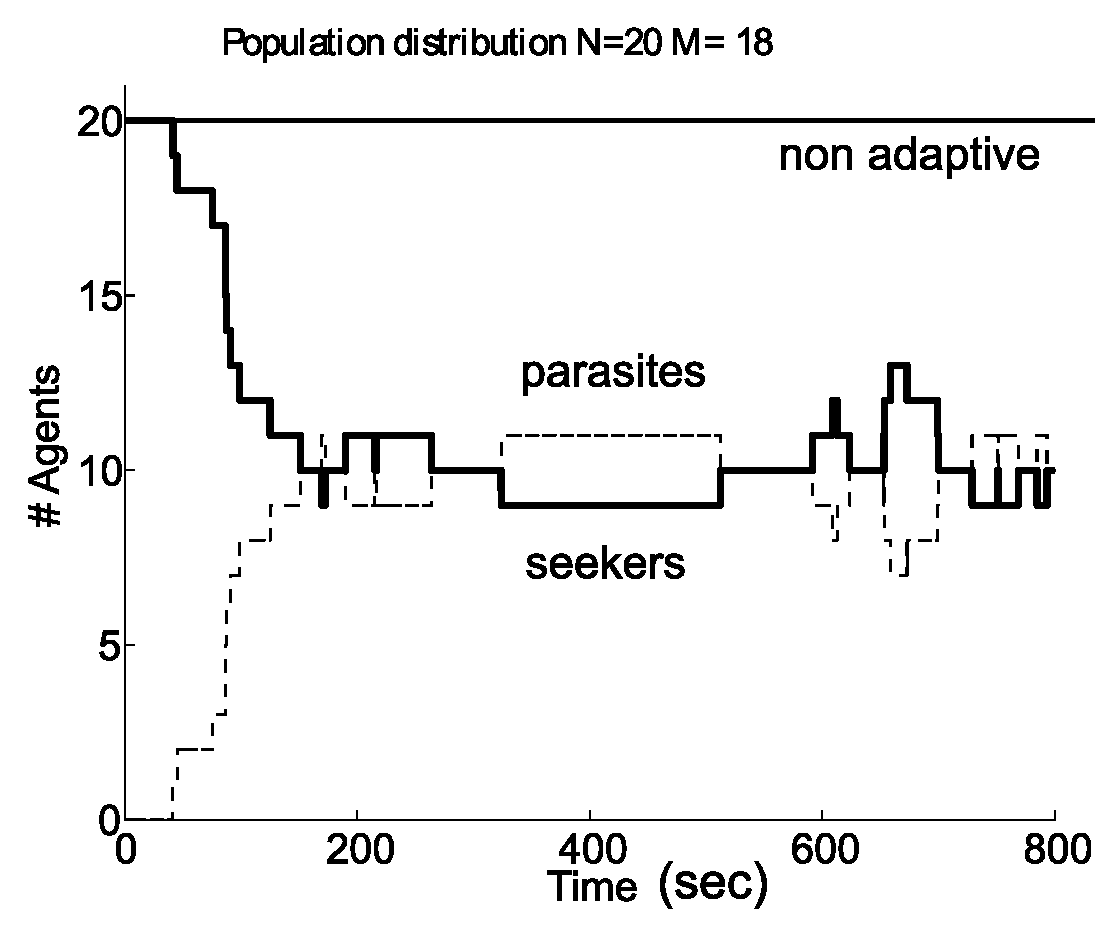
\includegraphics[width=0.4 \textwidth]{figures/socialadapt/honest/comm20TO18.eps}}
      \vspace{1pt}
      \subfigure[Dishonest food signal, ratio $N=20,M=4$, 18 cheaters]{
	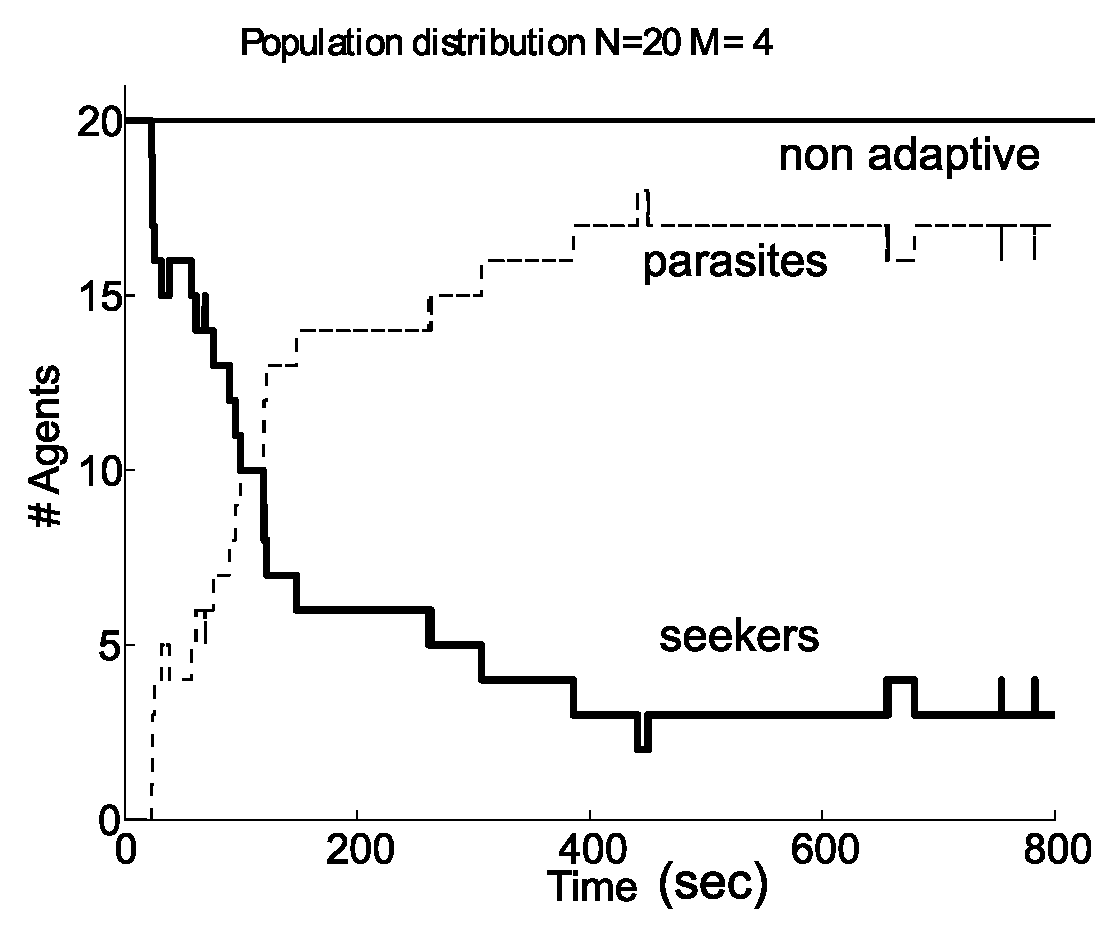
\includegraphics[width=0.4 \textwidth]{figures/socialadapt/deceptive/comm20TO4.eps}}
	\hspace{1pt}
      \subfigure[Dishonest food signal, ratio $N=20,M=16$, 18 cheaters]{
	\includegraphics[width=0.4 \textwidth]{figures/socialadapt/deceptive/comm20TO18.eps}}
    \caption[Sub system formation in different conditions]{
	  Population distribution in different cases: x-axis is the simulation time expressed in seconds,
	  y-axis reports the number of seekers $n_{s}(t)$ and of parasites $n_{p}(t)$ in function of time.
	  There are 6 diagrams, and for every diagram the adaptive communication
	  strategy versus the non communicative strategy is reported. \label{fig:generalcomparison}}
  \end{center}
\end{figure}

Considering the different cases in Fig.\ref{fig:generalcomparison}, it can be said that :
\begin{itemize}
\item in non-adaptive communication: parasites are absent (also with aggressive configuration see condition \ref{eq:aggressive} ), suggesting that adaptive communication is a necessary condition for the generation of sub-systems. In all cases (a) to (f): $n_{s}(t)=20$ and $n_{p}(t)=0$ at any time.
\item parasitism is a quasi-stable condition: the numbers of seekers and thus parasites stabilise after a transitory phase. For example in case (a) population distribution reaches an equilibrium: $n_{s}(t)=5\pm 1$ and $n_{p}(t)=15\pm$ with $t>400 s$. After 800 seconds (data not shown) the population distribution oscillates around the equilibrium.
\item the population dynamic is depending on the ratio between agents $N$ and food resources $M$:
\begin{itemize}
\item with scarce resources ($M=4$) in cases (a),(c),(e) parasites are prevalent
\item with abundant resources ($M=18$) in cases (d),(f) parasites are balanced with seekers, whereas in case (b) parasites are prevalent.
\end{itemize}
\end{itemize}
Table \ref{tab:population} resumes the stabilisation property of the population for 3 main cases:
\begin{enumerate}
\item silence: agents do not use the food social signal
\item honest: agents signal the food presence honestly
\item dishonest: some agents signals the food presence dishonestly, the rest of them do not signal (like the silence case)
\end{enumerate}

There are 2 important observations to make:
\begin{enumerate}
\item the ratio of seekers over parasites ($n_{s}/n_{p}$) depends non linearly to
the ratio of agents to food sources in the silence and dishonest cases. For example in
the silence scenario (agents do not signal the food presence) $n_{s}=5,3,5$
respectively for $M=4,10,18$. Interpolation techniques suggests that the dependency
is of exponential type.
\item the ratio of seekers over parasites ($n_{s}/n_{p}$) depends proportionally to the
ratio of agents to food sources in the honest case. Number of seekers $n_{s}$ increases
accordingly with the food sources $M$ such that $n_{s}=4,8,10$ respectively for $M=4,10,18$.
\end{enumerate}

\begin{table}[htbp]
\caption[Tabular results for self organisation property]{
Table summarising self-organisation:
every element in the table is the couple $(n_{s}(T_{sim}),n_{p}(T_{sim}))$
which indicates the number of seekers and parasites when the simulation
at the end of the simulation.\label{tab:population}}
\begin{center}
\small{
\begin{tabular}{@{}c|ccc@{}}
\hline
Ratio $N/M$ & 20:4 & 20:10 & 20:18\\
\hline
Silence & $(5,15)$ & $(3,17)$ & $(5,15)$\\
\hline
Honest & $(4,16)$ & $(8,12)$ & $(10,10)$\\
\hline
Dishonest agents:2  & $(7,13)$ & $(4,16)$ & $(8,12)$\\
Dishonest agents:10 & $(5,15)$ & $(6,14)$ & $(1,19)$\\
Dishonest agents:16 & $(10,10)$ & $(3,17)$ & $(8,12)$\\
\end{tabular}
}
\end{center}
\end{table}

A possible explanation for the prevalence of the parasitic population with scarce resources is due to the space constraints of the food sources: only a few agents (in our case 9) can forage at the same time, therefore the agents learn to transport food for the others. When resources are abundant this constraint is removed therefore the parasitic strategy is no longer needed.

\subsubsection{Foraging performance and signalling strategies}
If one wants to analyse the performance of the system in consuming food,
one could measure the number of the total bites can be measured:
\begin{equation}
 F_{tot}=F_{seek}+F_{parasite} \label{social:totbites}
\end{equation}
where $F_{seek}$ is the number of total times agents touched food sources (Eq. \ref{eq:touchfood})
and $F_{parasite}$ is the number of total times that agents touched other sated agents (Eq. \ref{eq:touchagent}).
Having chosen that index, table \ref{tab:totalPerformance} shows the $F_{tot}$ 
for the different conditions and underlines the value when dishonest is superior to 
the honest strategy.
On the basis of total bites, I can state that:
\begin{itemize}
\item honest signal is better then silence when food resources are $M=4,10,18$
\item comparing the honest and the dishonest strategy:
with 10 dishonest agents the $F_{tot}$ is superior to the honest one when $M=4,10$
but not when $M=18$. With only 2 dishonest agents, $F_{tot}$ is bigger only with scarce resources.
With 16 dishonest agents, performance is superior only in the intermediate case with $M=10$ resources.
\end{itemize}
It is also obvious that the dishonest strategy pays only when resources are scarce, 
which is also intuitive and has been shown in other simulation or
behavioural experiments such as \citet{Brembs1996:CheatingPrisonerDilemma,Schwieren2010:CompetitionCheating}.
The main idea is that if everybody is cheating and is not punished, the information
in the system is no more reliable and will punish everybody indiscriminately.

\begin{table}[htbp]
\caption[Social System foraging performance]{
Table summarising the foraging performance: every value represents $F_{tot}$. \label{tab:totalPerformance}}
\begin{center}
\small{
\begin{tabular}{@{}c|ccc@{}}
\hline
Ratio $N/M$ & 20:4 & 20:10 & 20:18\\
\hline
Silence & 373 & 347 & 371\\
\hline
Honest & 385 & 358 & 376\\
\hline
Dishonest agents:2 & \underline{391} & 348 & 343\\
Dishonest agents:10 & \underline{406} & \underline{385} & 339 \\
Dishonest agents:16 & 317 & \underline{369} & 351\\
\end{tabular}
}
\end{center}
\end{table}

Another index for the system performance is the equality in the food distribution. 
It means that, if I consider the mean $\mu$ and standard deviation $\sigma$ of 
the food bites over the $N=20$ agents, the food is better distributed ideally when 
the average $\mu$ is high as well as the deviation $\sigma$ is high. 
This indicate that a good distribution is when all agents in average have a good amount of food when the deviation
is high and average is high.
But if the average is high and the deviation is low, it means that few agents have
collected a large amount of food and thus is not desirable for a sustainable society.
Table \ref{tab:foodDistribution} contains the computed values for each condition.

\begin{table}[htbp]
\caption[Social System food distribution]{Table summarising food distribution:
every element represent the couple ($\mu,\sigma$) where $\mu$ is the average of
the food bites+agents bites over the agent population, and $\sigma$ is
the standard deviation. They are calculated at the end of the simulation.\label{tab:foodDistribution}}
\begin{center}
\small{
\begin{tabular}{@{}c|ccc@{}}
\hline
Ratio $N/M$ & 20:4 & 20:10 & 20:18\\
\hline
Silence & $(18.65,2.16)$ & $(17.35,2.83)$ & $(18.55,4.11)$\\
\hline
Honest & $(19.25,3.00)$ & $(17.90,2.51)$ & $(18,3.27)$\\
\hline
Dishonest (2 cheaters) & $(19.55,1.85)$  & $(17.40,2.09)$   & $(17.15,3.79)$\\
Dishonest (10 cheaters) & $(20.30,2.13)$  & $(19.25,2.63)$  & $(16.95,3.41)$\\
Dishonest (18 cheaters) & $(15.85,5.34)$ & $(18.45,2.58)$  & $(17.55,2.67)$\\
\end{tabular}
}
\end{center}
\end{table}

\begin{itemize}
\item for scarce resources $M=4$ and 2 cheaters: the best distribution comes 
with honesty:  $\mu_{honest}=19.25$ and $\sigma_{honest}=3.0$.
\item for scarce resources $M=4$ and 18 cheaters: dishonest has a smaller 
average  $\mu_{dishonest}=15.85$ but a better variance $\sigma_{honest}=5.34$ 
compared to the silence and honest strategy which has respectively a $\sigma_{silence}=2.16$ 
and $\sigma_{honest}=3.00$.
\item for abundant resources the honest and silence strategies are nearly equal, 
but with silence the variance is bigger $\sigma_{silence}=4.11)\sigma_{honest}=3.27$.
\item for abundant resources and any percentage of cheaters the honest strategy 
has the larger mean $\mu_{honest}=18.3$ and a comparable variance.
\end{itemize}


\subsubsection{Adaptive vs non communicative foraging performance}
In this scenario the honest communication strategy is compared to the non 
communicative behaviour. In figure \ref{fig:foraging1} it is reported the  
the number of total bites $F_{tot}$ (see Eq. \ref{social:totbites}) on the y-axis
in function of the simulation time on the x-axis for two cases: 
adaptive and non communicative strategy when the agents use the social honest signal. 
In case (a), where resources are scarce, before the sub-systems are formed 
(before $1x10^{4}$) $F_{tot}$ is equal in both cases, but during learning and, 
furthermore when the agents organise, the adaptive case overcomes the non
 adaptive one. In case (b), where resources are abundant, $F_{tot}$ is 
equal during all the time, because a strategy to optimize the food gathering
 is not essential.

\begin{figure}[htbp]
\begin{center}
\includegraphics[scale=0.3]{figures/socialadapt/foraging1.eps}
\end{center}
\vspace*{4pt}
\caption[Foraging performance comparison]{Foraging performance comparison:
thick line is the adaptive communication with honest signalling and the
dotted line is the non-adaptive communication case with honest signalling.
\textbf{Case (a):} scarce resources adaptive communication win.
\textbf{Case (b):} abundant resources, performances are equal
\label{fig:foraging1}}
\end{figure}


\subsubsection{Honest behaviour and unlimited resources}
In this scenario the agent honestly signals the presence of food places which
always produce the $G_{food}$ potential.
For this simulation, a population of $N=20$ agents is provided with $M=4,10,18$
food places sequentially. Population dynamic is observed for a total duration
of  $T_{sim}=80000$ (time step $\triangle T=0.01 seconds$).
Figure. \ref{fig:comparison} reports the number of seekers (thick line) and
parasites (dotted line) in function of time. 
The number of seekers $n_{s}(t)$ is complementary to the number of parasites 
$n_{p}(t)$: $n_{s}(t)+n_{p}(t)=N$.
The population ratios of seeker to parasites ($r(T_{sim})$) at the end of the
 simulation for every case $M=4,10,18$ are respectively $r(T_{sim})=4/16,8/12$ and $10/10$.
\begin{itemize}
\item in non-adaptive communication: parasites are absent (also with aggressive configuration see \ref{eq:aggressive}), suggesting that adaptive communication is a necessary condition for the generation of sub-systems.
\item in adaptive communication parasitism is a quasi-stable condition. With scarce resources ($M=4$), after 600 seconds, the number of seekers (see Fig. \ref{fig:comparison} (a)) stabilises to 4. With abundant resources ($M=18$), after 600 seconds, the number of seekers (see Fig. \ref{fig:comparison} (b)) stabilises to 10. After 800 seconds (data not shown) small oscillations around the stable point occur in both cases, suggesting that the system has reached an attractor.
\item the population ratio between seekers and parasites $r(T_{sim})$ depends on the ratio between the number of robots and the number of food places $N/M$:
\begin{itemize}
\item with scarce resources ($M=4$) parasites are prevalent: $n_{p}(T_{sim})=16\pm1 > n_{s}(T_{sim})=4\pm1$.
\item with abundant resources ($M=18$) seekers and parasites are in dynamical equilibrium (oscillate around the stable point after $T_{sim}$ steps): $n_{p}(T_{sim})=10\pm1$ and $n_{s}(T_{sim})=10\pm1$.
\end{itemize}
\end{itemize}
An explanation for the prevalence of the parasitic population with scarce resources is due to the space constraints of the food sources: only a few agents (in our case 9) can forage at the same time, therefore agents "transport" food for the others. When resources are abundant this constraint is removed therefore parasitism is not essential.

\begin{figure}[ht]
  \begin{center}
      \subfigure[Case considering scarce resources: in non adaptive-communication only seekers are present (top line is constant to 20 agents), in adaptive communication sub-system formation is achieved and parasites become more than seekers after 80 seconds]{
	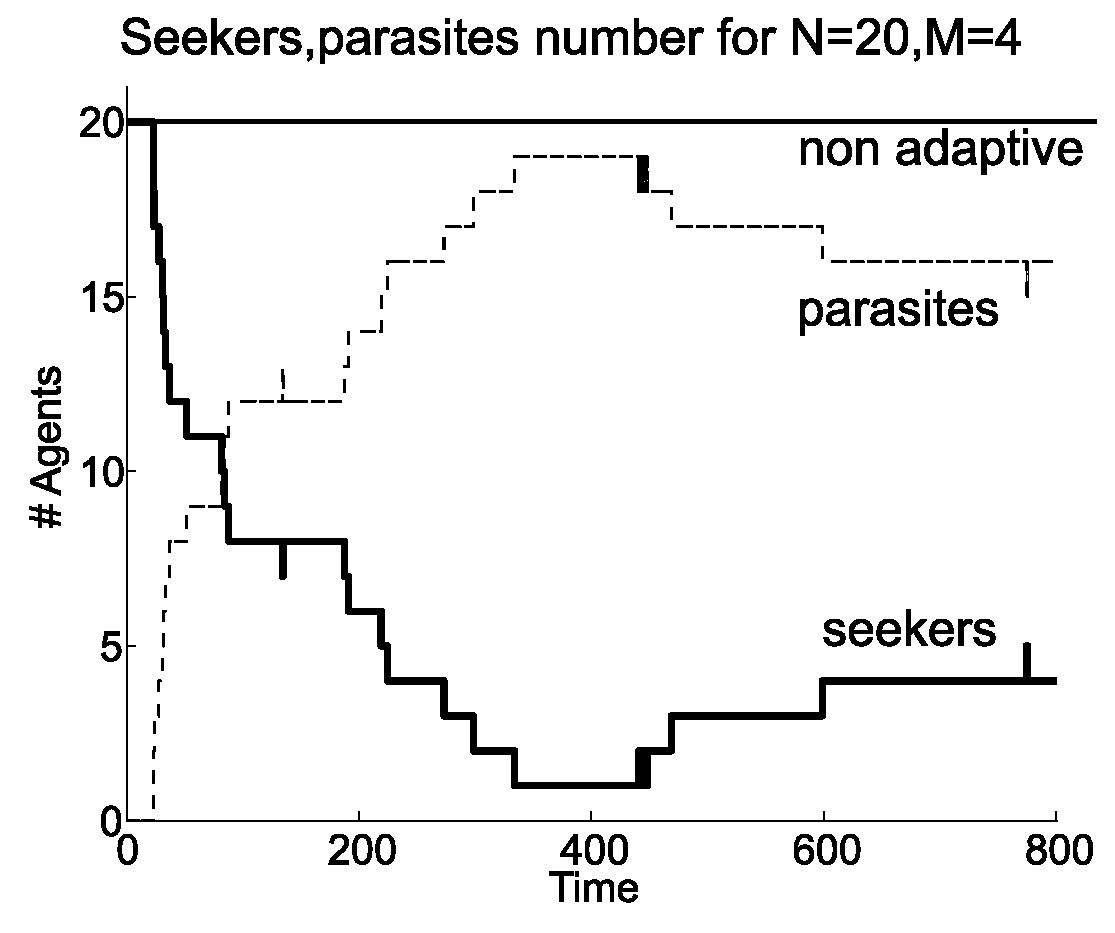
\includegraphics[width=0.4 \textwidth]{figures/socialadapt/20to4.eps}}
	\hspace{1pt}
      \subfigure[Case considering scarce resources: in non adaptive-communication only seekers are present (top line is constant to 20 agents), in adaptive communication sub-system formation is achieved and parasites are in equilibrium with seekers after 200 seconds]{
	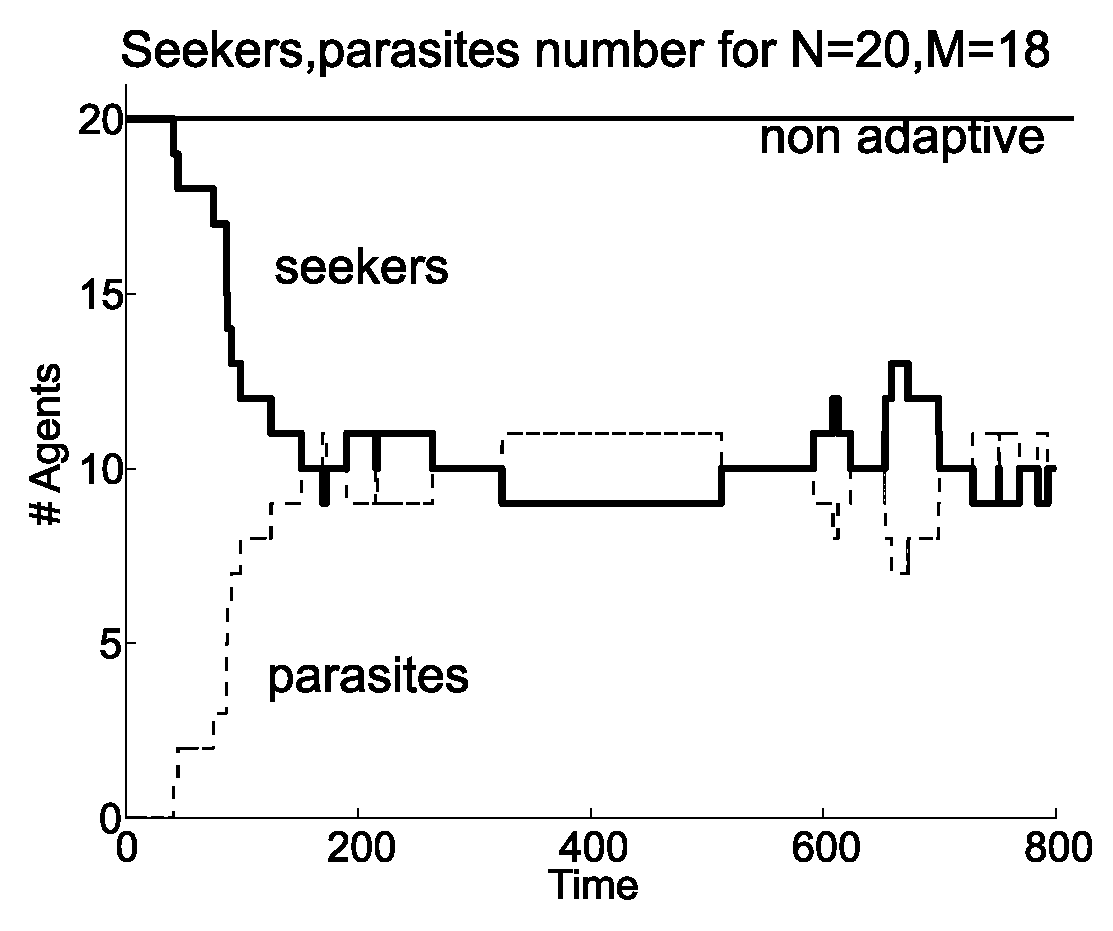
\includegraphics[width=0.4 \textwidth]{figures/socialadapt/20to18.eps}}
    \caption[Self organisation with honest behaviour and unlimited resources]{\label{fig:comparison}}
  \end{center}
\end{figure}
To analyse the performance of the system in consuming food: the number of the total bites $F_{tot}=F_{seek}+F_{parasite}$ it is considered.
$F_{seek}$ is the number of total times that agents touched food sources (Eq. \ref{eq:touchfood}) and $F_{parasite}$ is the number of total times that agents touched other sated agents (Eq. \ref{eq:touchagent}). In table \ref{tab:performance} it is reported the foraging performance (average $\pm$ range) over 100 simulations and it can be noticed that adaptive communication provides the best performance only for scarce resources and an equal performance for abundant resources.

\begin{table}[htbp]
\caption[Foraging performance with unlimited resources]{
Table summarising foraging performance over 100 simulations.
With scarce resources, performance is superior using adaptive communication,
with abundant resources performances are equal since food distribution
through parasites is not essential.\label{tab:performance}}
{
\begin{tabular}{@{}cccc@{}}
\hline
Ratio $N/M$ & 20:4 & 20:18\\
\hline
Adaptive communication & $F_{tot}=396\pm2$ & $F_{tot}=319\pm2$\\
\hline
Non-adaptive communication & $F_{tot}=355\pm2$ & $F_{tot}=319\pm2$\\
\hline
\end{tabular}}
\end{table}

\subsubsection{Honest behaviour and limited resources}
In this scenario the agent honestly signals the presence of food which is limited in time.
For this simulation, a population of $N=20$ agents is provided with $M=4,10,18$
food places sequentially. Population dynamic is observed for a total duration
of  $T_{sim}=80000$ (time step $\triangle T=0.01 seconds$).
The population ratios of seeker to parasites ($r(T_{sim})$) at the end of
the simulation for every case $M=4,10,18$ are respectively $r(T_{sim})=5/15,8/12$
and $10/10$.
\begin{itemize}
\item in non-adaptive communication: parasites are absent (also with aggressive
configuration see \ref{eq:aggressive}), suggesting that adaptive communication
is a necessary condition for the generation of sub-systems.
\item in adaptive communication parasitism is a quasi-stable condition.
With scarce resources ($M=4$), after 600 seconds, the number of seekers
(see Fig. \ref{fig:limitedcomparison} (a)) stabilize to 5. With abundant resources ($M=18$),
after 600 seconds, the number of seekers (see Fig. \ref{fig:limitedcomparison} (b))
stabilises to 10. After 800 seconds (data not shown) small oscillations around
the stable point occur in both cases, suggesting that the system has reached an attractor.
\item the population ratio between seekers and parasites $r(T_{sim})$ depends
on the ratio between the number of robots and the number of food sources $N/M$:
\begin{itemize}
\item with scarce resources ($M=4$) parasites are prevalent:
$n_{p}(T_{sim})=15\pm1$ $>$ $n_{s}(T_{sim})=5\pm1$.
\item with abundant resources ($M=18$) seekers and parasites are in dynamical
equilibrium (oscillate around the stable point after $T_{sim}$ steps):
$n_{p}(T_{sim})=10\pm2$ and $n_{s}(T_{sim})=10\pm2$.
\end{itemize}
\end{itemize}

\begin{figure*}
\centerline{\subfigure[Case considering scarce resources: in non adaptive-communication
 only seekers are present (top line is constant to 20 agents), in adaptive communication
 sub-system formation is achieved and parasites become more than seekers after 200 seconds]{
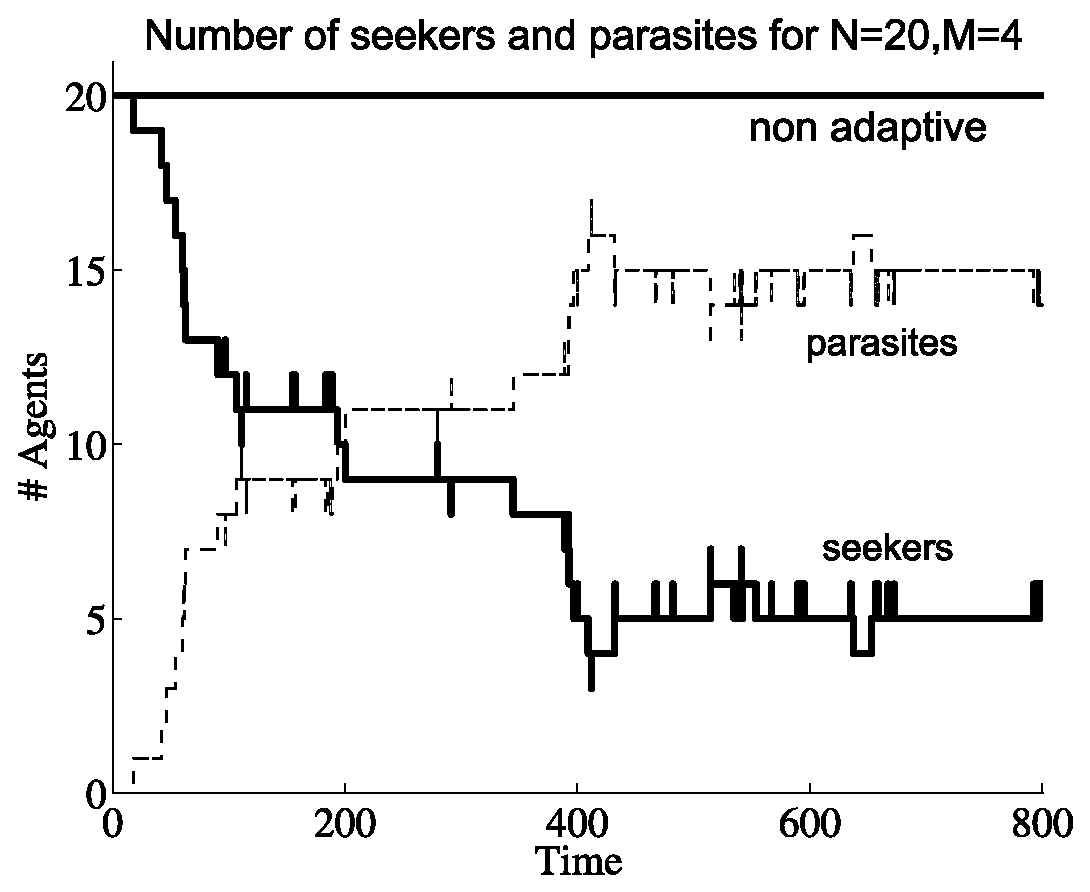
\includegraphics[width=2.4in]{figures/socialadapt/limited/20to4.eps}
\label{fig_first_case}}
\hfil
\subfigure[Case considering scarce resources: in non adaptive-communication
only seekers are present (top line is constant to 20 agents), in adaptive
communication sub-system formation is achieved and parasites are in equilibrium
with seekers after 200 seconds]{
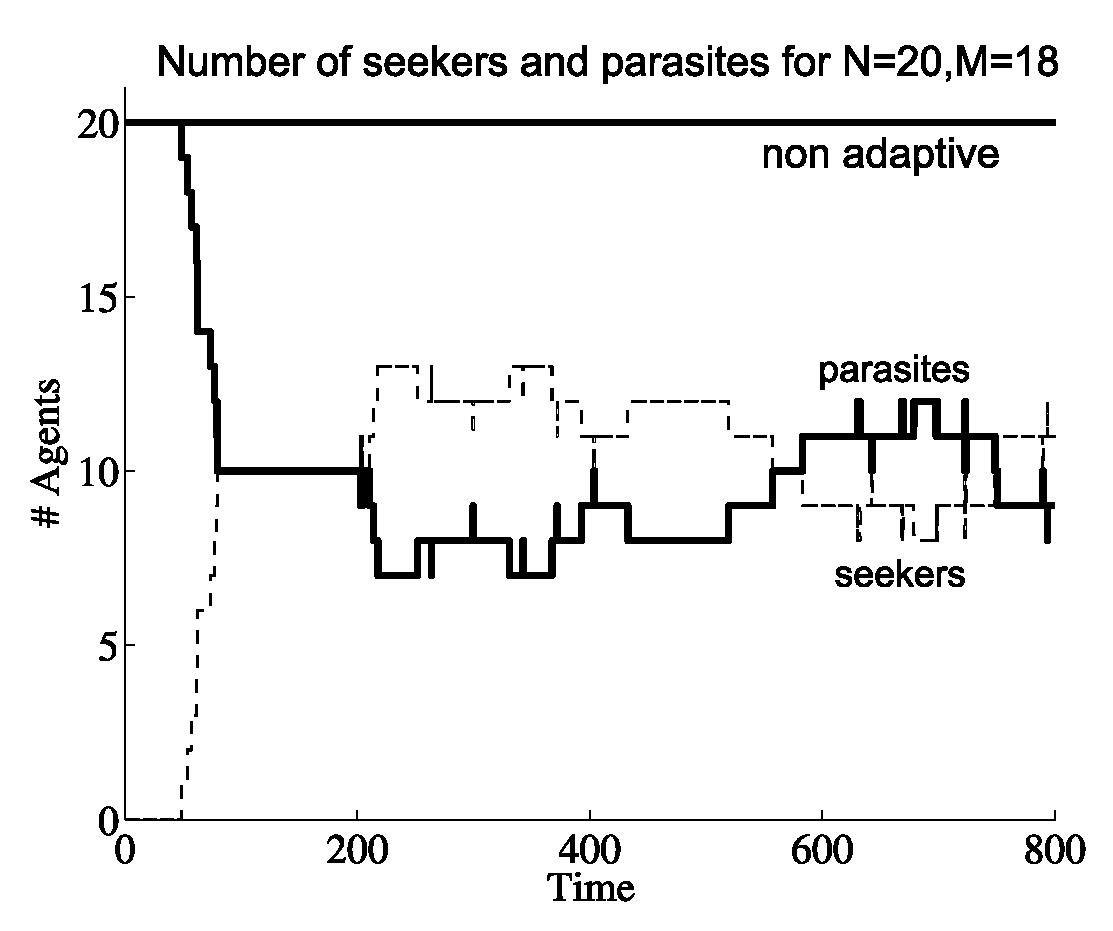
\includegraphics[width=2.4in]{figures/socialadapt/limited/20to18.eps}
\label{fig_second_case}}}
\caption[Self organisation with honest behaviour and limited resources]{Self organisation with honest behaviour and limited resources\label{fig:limitedcomparison}}
\label{fig_sim}
\end{figure*}
An explanation for the prevalence of the parasitic population with scarce
resources is due to the space constraints of the food places: only few agents
 (in our case 9) can forage at the same time, therefore agents "transport"
food for the others. When resources are abundant this constraint is
removed therefore parasitism is not essential.

To analyse the performance of the system in consuming food: the number of the total
bites $F_{tot}=F_{seek}+F_{parasite}$ it is considered.
$F_{seek}$ is the number of total times that agents touched food sources
(Eq. \ref{eq:touchfood}) and $F_{parasite}$ is the number of total times that
agents touched other sated agents (Eq. \ref{eq:touchagent}).
In table \ref{tab:limitedperformance} the foraging performance
(average $\pm$ range) over 100 simulations is demonstrated and it can be noticed that adaptive
communication provide the best performance in term of food foraging for scarce
and abundant resources. Why is the performance better than the unlimited case?
Because this time the food resources are limited in time and space, so even when
 there are a lot of food resources the agents must collaborate to maximise
the food collection.

\begin{table}
%% increase table row spacing, adjust to taste
\renewcommand{\arraystretch}{1.3}
\caption[Foraging performance with limited resources]{
Table summarising foraging performance over 100 simulations.
Adaptive communication has the best performance for both scarce
and abundant resources.\label{tab:limitedperformance}}
\begin{center}
\begin{tabular}{@{}cccc@{}}
\hline
\hline
Ratio $N/M$ & 20:4 & 20:18\\
\hline
Adaptive communication & $F_{tot}=439\pm2$ & $F_{tot}=340\pm2$\\
\hline
Non-adaptive communication & $F_{tot}=320\pm2$ & $F_{tot}=230\pm2$\\
\end{tabular}
\end{center}
\end{table}

\subsubsection{Stability analysis for changes in population}
Every self organizing system should be stable to external variations in the 
parameter space, this property is generally known as robustness to variation.
If the number of agents are changed during simulation the system reacts promptly
and stabilize to a new state. In Fig.\ref{fig:agentAdd} seekers are stabilised
in the range $4\pm1$, when 6 more agents are added at time 400,
seekers stabilize again in the range $7\pm1$

\begin{figure}[htb]
\begin{centering}
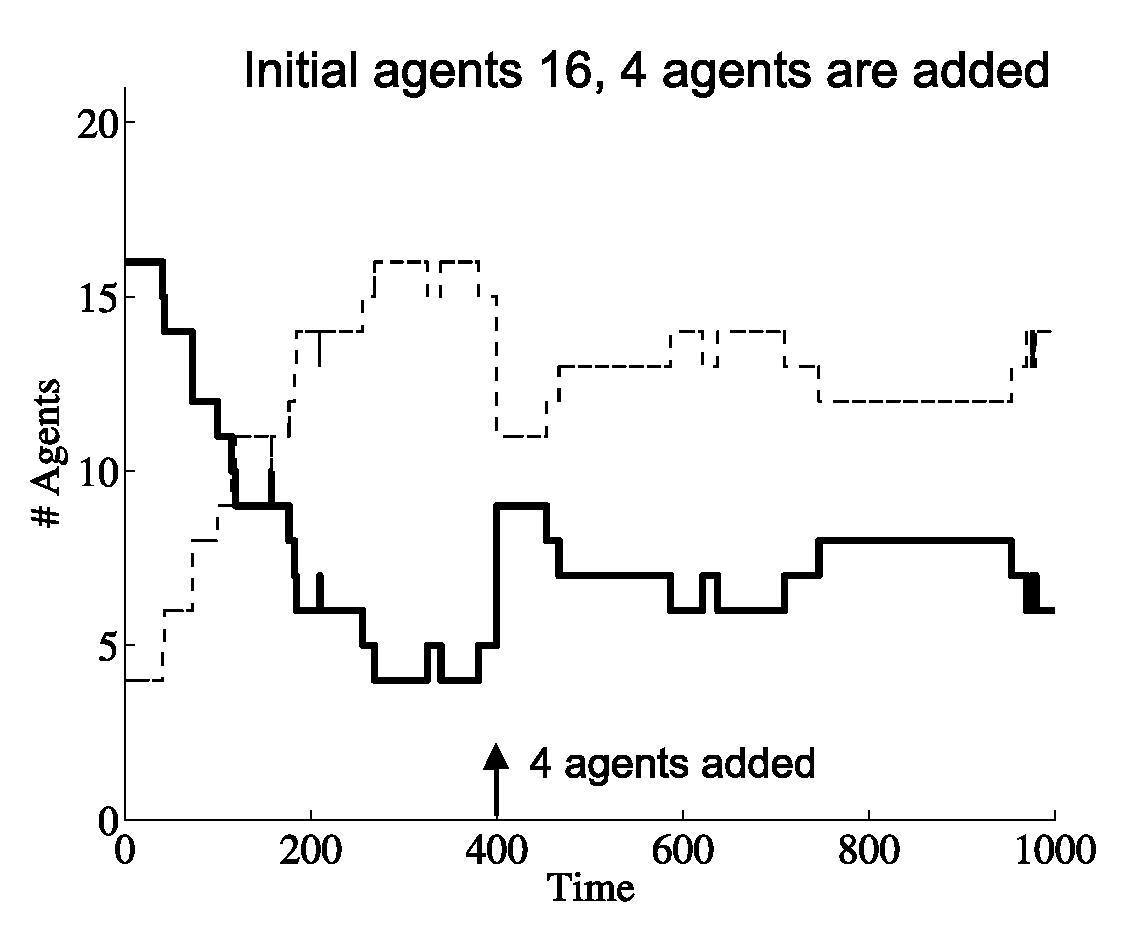
\includegraphics[width=0.6 \textwidth]{figures/socialadapt/limited/agent4more.eps}
\small{
\caption[Self organisation sensitivity to agent parameters]{
Simulation starts with 16 agents, then 4 agents are added
after 400 seconds.\label{fig:agentAdd}}
}
\end{centering}
\end{figure}

This property indicates that the system is robust to a variation in the number
of agents: the system will adjust automatically to the new equilibrium with a certain
response time.
The system is also robust to a variation in the food resources, although with 
a slower response time (not shown in the Figure).
This stability is a good feature especially for real implementation of 
social systems where disturbances from the environment are likely to occur
very often and the designer is certain that the system will be stable enough
to keep with the foraging task.


\subsection{Discussion: sub system formation in the social model}
The simulations of a social system based on pro-active learning agents has shown
very promising results.
First of all the system self-organizes by means of individual specialization 
to the environment conditions which are the number of agents and number of food resources.
Agents are based on a simple, yet effective learning mechanism called ICO which
can be extended to implement competitive behaviours.
Because internal processing is avoided, agents respond to the changes of their
environment in a timely fashion.
The system is able to generate sub-systems as Luhmann proposed by means of communication,
in absence of communication specialization is not possible.
Other embodiments for the learning controller could have been chosen, for instance
with Q-learning \citep{watkins92a} reactive agents are given a description of the
current state and have to choose the next action so as to maximise a scalar
reinforcement received after each action.
The task of the agent is to learn from indirect, delayed reward, to choose sequences of actions
that produce the greatest cumulative rewards. Reinforcement learning algorithms attempt to find
a policy that maps states of the world to the actions the agent ought to take in those states.
In economics and game theory, reinforcement learning is considered as a boundedly rational
interpretation of how equilibrium may arise. Reinforcement models for MAS suffers of 2 disadvantages:
\begin{enumerate}
\item complexity may be exponential in the number of environmental states.
\item discrete models: agents choose from a set of actions in a discretised world
\end{enumerate}
This problem is crucial in MAS: when an agent is learning the value of its actions
in the presence of other agents, it is learning in a non stationary environment.
In \citep{Qlearning-MAS} a novel exploration strategy, for
the Q-algorithm applied in a predator-prey game to obtain convergence, is introduced.
Unfortunately the cost of communication in their model is very expensive,
so they discuss only the case without communication.
Our learning rule ICO, is unsupervised and is computationally efficient (since it does not rely on states)
and inspired on the evidence that organism tends to maintain a weak homoeostasis
with the environment as demonstrated by \citet{McFarland93}.
In \citep{tan97multiagent} Q-learning is applied in a predator-prey game,
where agents cooperate in different ways. It is interesting to analyse the
communication method called sharing sensation. The model is composed of 1 hunter,
1 prey and a scouting agent. At each step, the scout sends its action and sensation
back to the hunter: the hunter relies initially on his sensation and
then on the scout's sensation. Therefore the scout can be compared in our model
 as the distal signal: hunter can see the prey at longer distances.
Performance (number of steps to capture a prey) is then compared in the 2 cases:
scouting versus no scouting. Performance is superior in the scouting case
,as well as in our model performance, it is superior when agents use both
proximal and distal signal (see table \ref{tab:performance}).
Another approach used to develop communication in MAS is in \citet{Floreano-MAS}
where a genetic-algorithm is used to evolve 1000 robots (divided in 100 colonies).
The control system used is a feed-forward neural network with 10 inputs and 3 output neurons.
The network was encoded using a genetic string of 240 bits. Synaptic weights are only
evolved and not learned and robots had a sensory-motor cycle of 50 ms.
Our controller makes use of 12 inputs (2 more) and 2 motor neurons + 1 the
$G_{satedness}$ signal, but does not use a sensory-motor cycle allowing fast responses.
Thus \citet{Floreano-MAS} makes use of genetic selection and recombination to produce
robots behaviours (communication strategies). Hence the agent system do not self organise
in classes.
Other similar works, making use of evolved recurrent neural networks
(RNNs \nomenclature{RNN}{Recurrent Neural Networks})
are reported in \citet{EmergenceCommMas} and \citet{OriginsComm}. In \citet{OriginsComm}
a population of agents evolved for the ability to solve a collective navigation problem
develop individual and social/communication skills. A particular evolved behaviour
resembles our system differentiation: ``a differentiation of the modalities with
which communication is regulated (... e.g. specialised asymmetrical interaction
forms in which one robot acts as a speaker and one robot acts as an hearer)''.
In \citep{EmergenceCommMas} the evolutionary adaptivity of RNNs to
varying environmental conditions, such as the number of interacting robots is studied.
In my model the system specializes in a group that gets the food and distributes it (seekers) and
the other one (parasites) collects it.
The communication strategy was robust only for small changes. In our model,
agents adapt continuously to the environment, they self-organise efficiently
with varying robot number $N$ and varying $M$ food sources.
Moreover the system converges to a quasi-stable state thanks to the stability
provided by the learning rule.
The system performance in terms of food foraging behaviour was analysed for 
a honest and dishonest signalling strategy both in terms of food distribution
and in terms of total energy acquired.
This study can be used to predict the performance of a social robotic system in
a real test case so that the designer can choose the parameters according to the
desired performance.
In the following sections, I will introduce input measures that quantify the
agent performance and information selection as suggested by Luhmann. 





